\documentclass[10pt, a4paper, ngerman]{arbeitsblatt}

\ladeModule{theme,boxen}

\ladeFach[uml]{informatik}

\aboptionen{
	name		= {J. Neugebauer},
	kuerzel		= {Ngb},
	titel		= {Cheese Champion},
	reihe		= {Lineare dynamische Datenstrukturen},
	fach		= {Informatik},
	lerngruppe	= {Q1},
	nummer		= {II.06},
	lizenz		= {cc-by-nc-sa-4},
	version		= {2022-09-21},
}

\begin{document}
\ReiheTitel

\textbf{Cheese Champion} (dt. \emph{Mäusekampf}) ist der Titel einer Aufgabe aus dem \emph{17. Bundeswettbewerb Informatik}.
\begin{rahmen}\small
\begin{wrapfix}
	\begin{wrapfigure}{r}{4cm}
		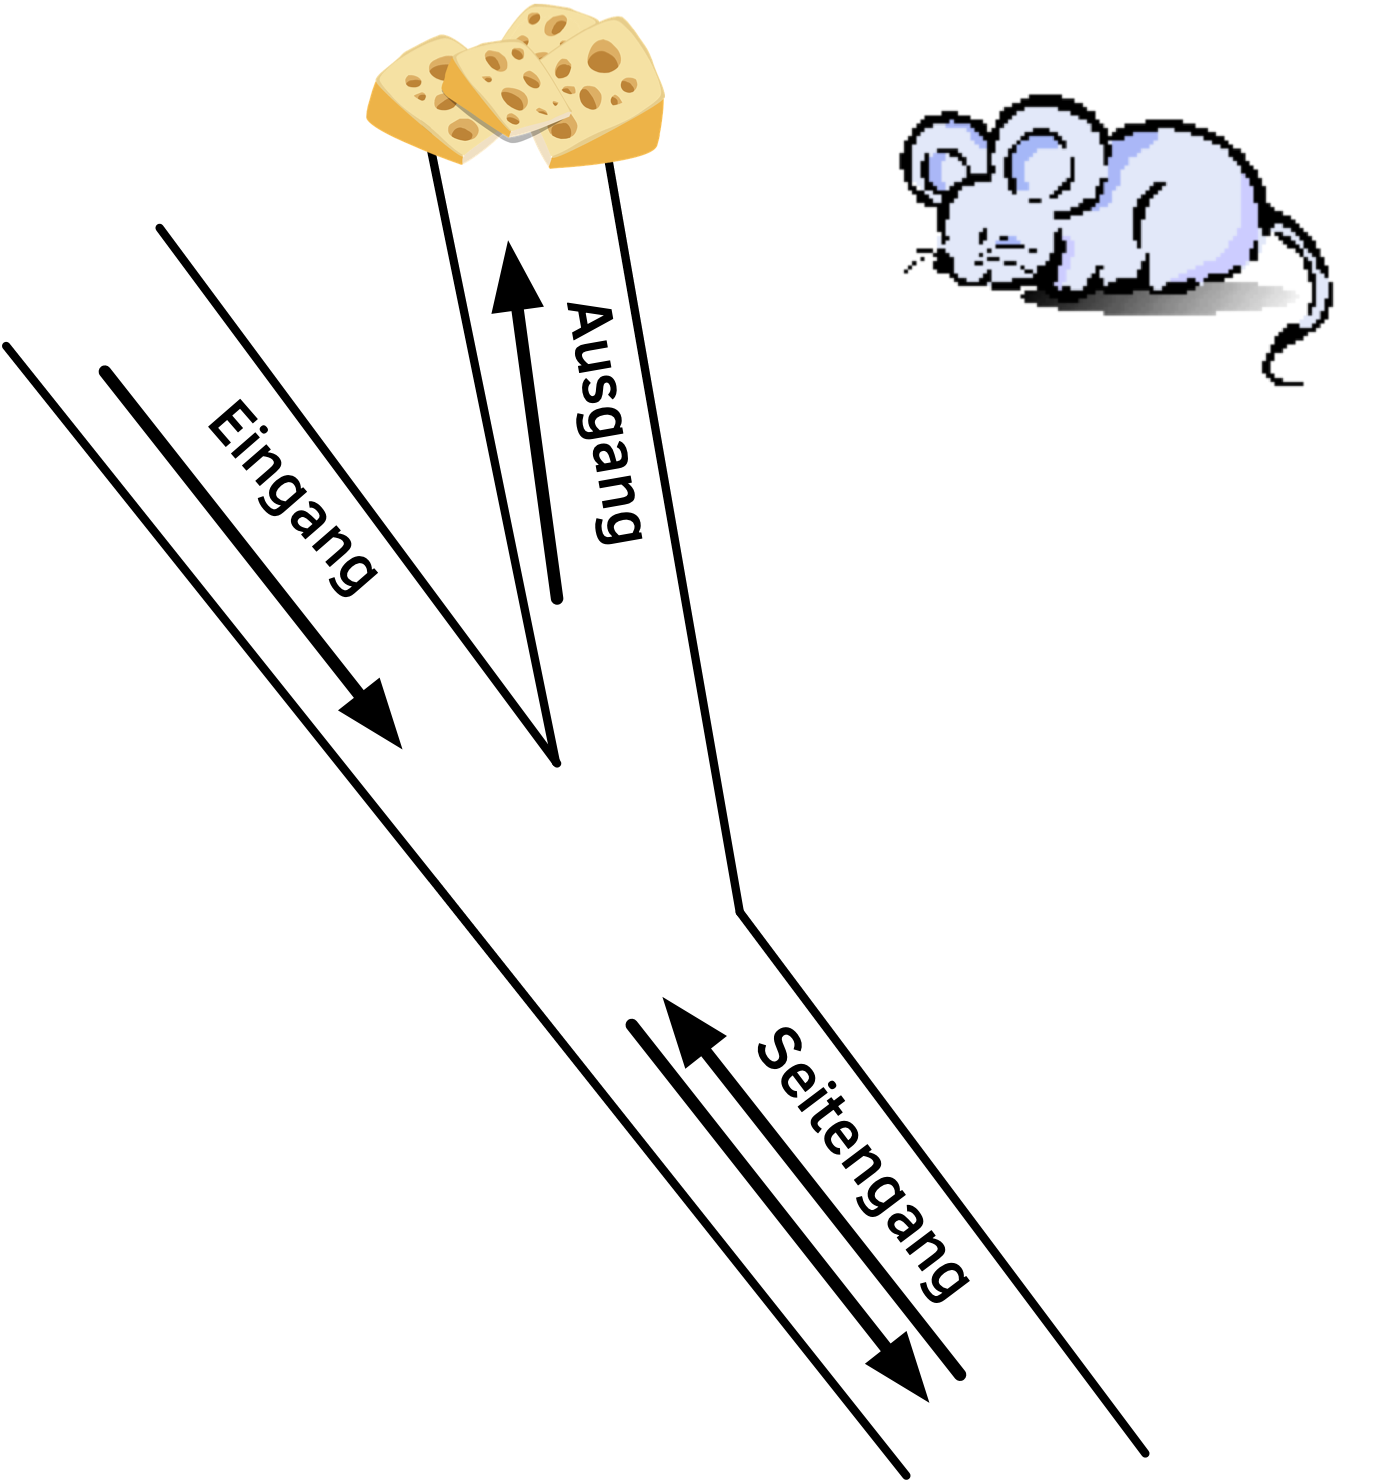
\includegraphics[width=4cm]{Q1-AB.II.06-Cheese_Champion.png}
	\end{wrapfigure}

	Prof. Grip will die Durchsetzungsfähigkeit einzelner Mäuse einer Mäusekolonie feststellen. Dazu hat er die folgende Versuchsanordnung entworfen: Ausgehend von einem unterirdischen Gang gräbt er einem spitzen Winkel einen Ausgang zur Oberfläche, an dessen Ende er einen Stück duftenden Käse deponiert.

	Die Mäuse der Kolonie kommen direkt hintereinander von links in den unterirdischen Gang und wollen durch den Abzweig zum Käse. Da der Gang zum Käse in einem spitzen Winkel abzweigt, muss jede Maus erst über den Abzweig hinaus weiter in den Gang hineinlaufen. Dann dreht sie sich um und hat möglicherweise ein Problem: Sie stößt auf die nachfolgende Maus, die ebenfalls in den rechten Abschnitt möchte.

	Präziser gelten folgende Regeln für das Erreichen des Käses:
	\begin{smallitem}
		\item Jede Maus aus dem Eingang muss zunächst an der Abzweigung vorbei in den Seitengang.
		\item Wenn Sie im Seitengang ist, dann kann Sie entweder den Zweikampf gegen die nachfolgende Maus aus dem Eingang gewinnen und so zum Ausgang gelangen, oder sie wird von der Gewinnerin tiefer in den unterirdischen Gang gedrängt. Die Gewinnerin betritt nun ihrerseits den Seitengang und kämpft gegen die nachfolgende Maus aus dem Eingang.
		\item Befinden sich keine Mäuse mehr im Eingang, dann können die verbliebenen Mäuse im Seitengang direkt zum Ausgang gehen.
	\end{smallitem}

	Prof. Grips nummeriert die Mäuse in der Reihenfolge, in der sie in den Gang hineinlaufen, mit 1, 2, 3, ... und beobachtet, in welcher Reihenfolge sie beim Käse ankommen.
\end{wrapfix}
\end{rahmen}

\begin{aufgabe}
\begin{teilaufgaben}
	\teilaufgabe
	In der Versuchsanordnung von Prof. Grips gibt es drei Gänge: den Eingang, den Seitengang und den Ausgang. Entscheide jeweils, welche lineare dynamische Datenstruktur jeweils am besten geeignet ist.

	\teilaufgabe
	Spiele den \enquote{Mäusekampf} mit folgenden vier Mäusen durch. In welcher Reihenfolge erreichen sie den Käse?

	\begin{multicols}{4}
		Maus 1 (Stärke 5)

		Maus 2 (Stärke 8)

		Maus 3 (Stärke 4)

		Maus 4 (Stärke 10)
	\end{multicols}

	Überlege dir mögliche Sonderfälle im Ablauf des Kampfes. (Was ist zum Beispiel, wenn der Seitengang leer ist?)

	\teilaufgabe
	Das folgende \emph{Entwurfsdiagramm} zeigt die Klassen eines \code{CheeseChampion}-Programms.

	\begin{center}
		\begin{klassendiagramm}
			\begin{class}[text width=3cm]{CheeseChampion}{0,0}
				\operation{kampf}
				\operation{erzeugeMaeuse}
			\end{class}
			\begin{class}[text width=3cm]{Maus}{10,0}
				\attribute{nummer : Zahl}
				\attribute{staerke : Zahl}
			\end{class}
			%% Assoziationen manuell zeichnen
			\draw[umlcd style,->] (CheeseChampion.north east) --node[above,sloped,black,label=below:0..*]{eingang} (Maus.north west);
			\uses{CheeseChampion}{seitengang}{0..*}{Maus}
			\draw[umlcd style,->] (CheeseChampion.south east) --node[above,sloped,black,label=below:0..*]{ausgang} (Maus.south west);
		\end{klassendiagramm}
	\end{center}

	In Gitea befinden sich drei Versionen des Projekts, die aufsteigend immer konkretere Hilfen zur Implementierung enthalten. Entscheide dich für eine der drei Versionen und implementiere die Simulation des Mäusekampfes entsprechend der Regeln oben.

	Beginne mit der Klasse \code{Maus}, sofern diese noch nicht vollständig implementiert ist.

	\teilaufgabe
	Implementiere als Erweiterung eine Methode, die anhand einer beobachteten Reihenfolge (als Schlange gegeben) prüft, ob diese Reihenfolge tatsächlich aus einem Mäusekampf hervorgegangen sein kann. (Simuliere dazu den Kampf \enquote{rückwärts}.)
\end{teilaufgaben}
\end{aufgabe}

\end{document}
